% !TeX spellcheck = cs_CZ
%{\tikzset{external/prefix={tikz/FYZII/}}
% \tikzset{external/figure name/.add={ch36_}{}}
%---------------------------------------------------------------------------------------------------
% file fey2ch36.tex
%---------------------------------------------------------------------------------------------------
%=========================== Kapitola Feromagnetizmus ==============================================
\setchaptertoc
\chapter{Feromagnetizmus}\label{fyz:IIchapXXXVI}

  \section{Magnetizační proudy}\label{fyz:IIchapXXXVIsecI}
  \section{Pole H}\label{fyz:IIchapXXXVIsecII}
  \section{Magnetizační křivka}\label{fyz:IIchapXXXVIsecIII}
  \section{Indukčnost ocelových jader}\label{fyz:IIchapXXXVIsecIV}
  \section{Elektromagnety}\label{fyz:IIchapXXXVIsecV}
  \section{Spontánní magnetizace}\label{fyz:IIchapXXXVIsecVI}
  \section{Příklady a cvičení}\label{fyz:IIchapXXXVIsecVII}

    \begin{figure}[ht!] %\ref{fyz:fig0831}
      \centering
      \subcaptionbox{\label{fyz:fig0831a}}{\luafigure[0.9]{fyz_fig0831a.pdf}}               \\
      \subcaptionbox{\label{fyz:fig0831b}}{\luafigure[0.9]{fyz_fig0831b.pdf}}               \\
      \subcaptionbox{\label{fyz:fig0831c}}{\luafigure[0.9]{fyz_fig0831c.pdf}}
      \caption{
               (\cite[s.~748]{Feynman02})}
      \label{fyz:fig0831}
    \end{figure}

    \begin{figure}[ht!] %\ref{fyz:fig0832}
      \centering
      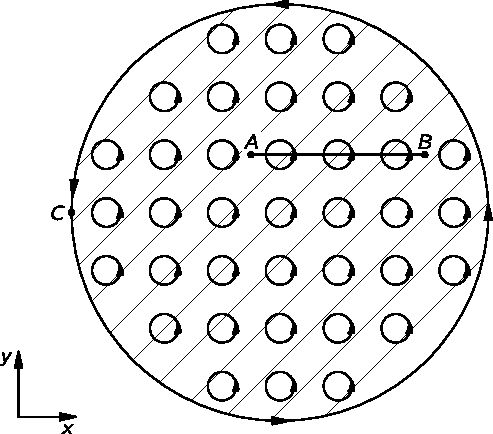
\includegraphics[width=0.7\linewidth]{fyz_fig0832.pdf}
      \caption{
               (\cite[s.~707]{Feynman02})}
      \label{fyz:fig0832}
    \end{figure}
    
    \begin{figure}[ht!] %\ref{fyz:fig0833}
      \centering
      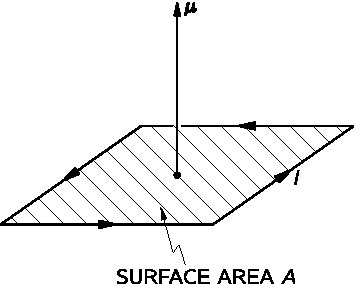
\includegraphics[width=0.7\linewidth]{fyz_fig0833.pdf}
      \caption{
               (\cite[s.~707]{Feynman02})}
      \label{fyz:fig0833}
    \end{figure}
    
    \begin{figure}[ht!] %\ref{fyz:fig0834}
      \centering
      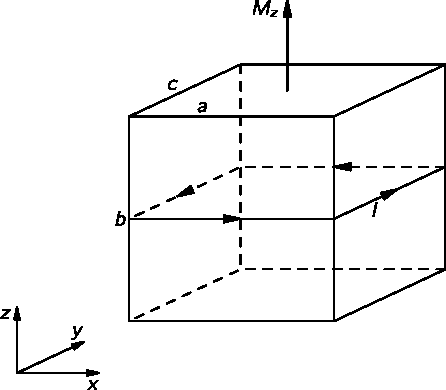
\includegraphics[width=0.7\linewidth]{fyz_fig0834.pdf}
      \caption{
               (\cite[s.~707]{Feynman02})}
      \label{fyz:fig0834}
    \end{figure}
    
    \begin{figure}[ht!] %\ref{fyz:fig0835}
      \centering
      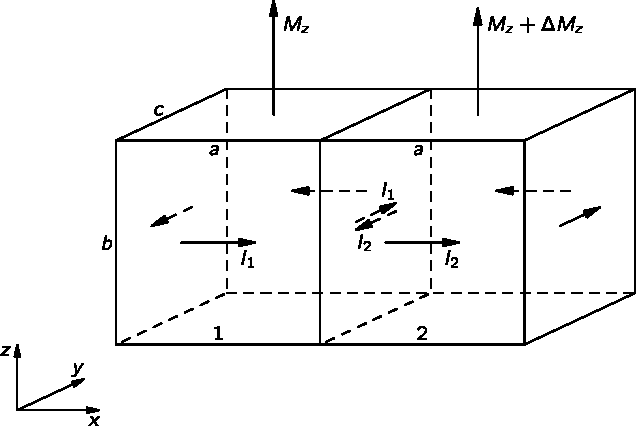
\includegraphics[width=0.7\linewidth]{fyz_fig0835.pdf}
      \caption{
               (\cite[s.~707]{Feynman02})}
      \label{fyz:fig0835}
    \end{figure}
    
    \begin{figure}[ht!] %\ref{fyz:fig0836}
      \centering
      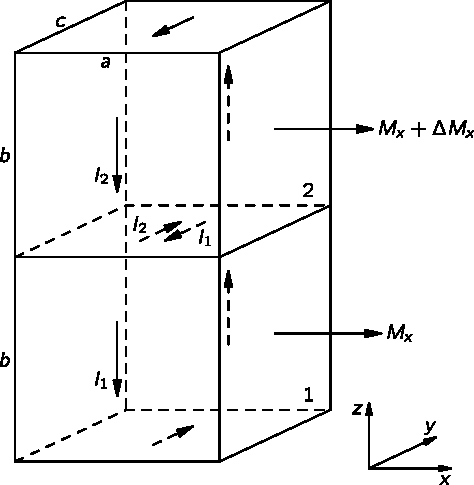
\includegraphics[width=0.7\linewidth]{fyz_fig0836.pdf}
      \caption{
               (\cite[s.~707]{Feynman02})}
      \label{fyz:fig0836}
    \end{figure}

    \begin{figure}[ht!] %\ref{fyz:fig0837}
      \centering
      \subcaptionbox{\label{fyz:fig0837a}}{\luafigure[0.9]{fyz_fig0837a.pdf}}               \\
      \subcaptionbox{\label{fyz:fig0837b}}{\luafigure[0.9]{fyz_fig0837b.pdf}}
      \caption{
               (\cite[s.~748]{Feynman02})}
      \label{fyz:fig0837}
    \end{figure}

    \begin{figure}[ht!] %\ref{fyz:fig0838}
      \centering
      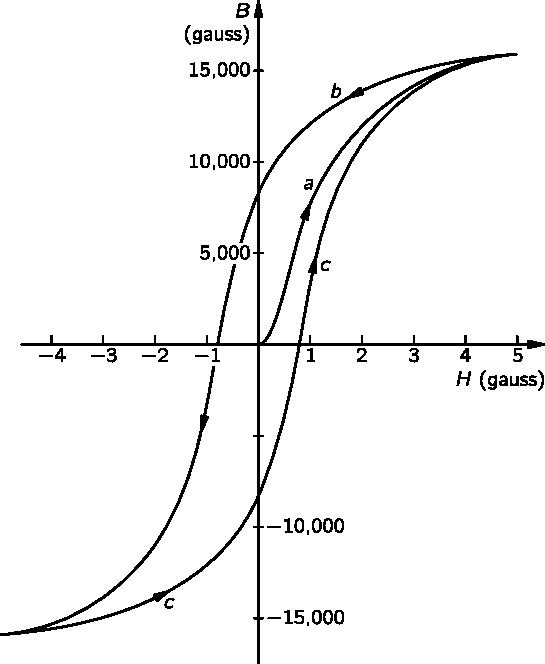
\includegraphics[width=0.7\linewidth]{fyz_fig0838.pdf}
      \caption{
               (\cite[s.~707]{Feynman02})}
      \label{fyz:fig0838}
    \end{figure}

    \begin{figure}[ht!] %\ref{fyz:fig0839}
      \centering
      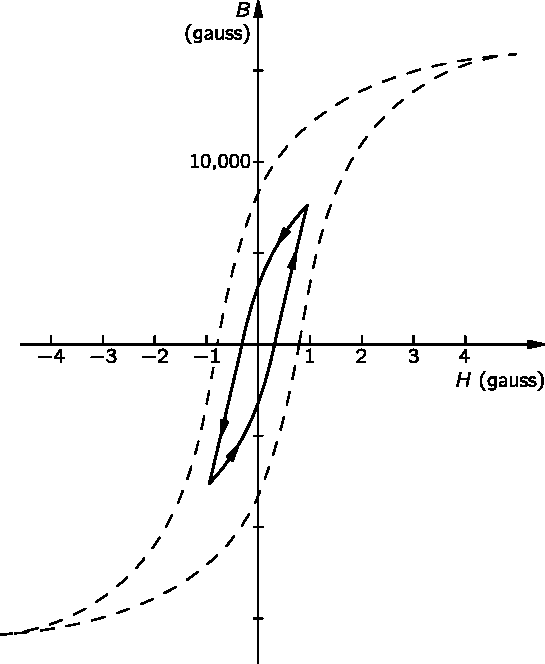
\includegraphics[width=0.7\linewidth]{fyz_fig0839.pdf}
      \caption{
               (\cite[s.~707]{Feynman02})}
      \label{fyz:fig0839}
    \end{figure}

    \begin{figure}[ht!] %\ref{fyz:fig0840}
      \centering
      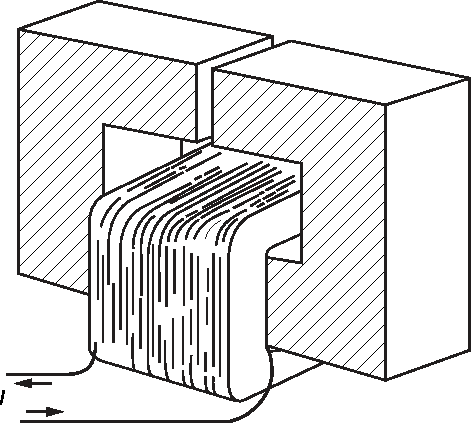
\includegraphics[width=0.7\linewidth]{fyz_fig0840.pdf}
      \caption{
               (\cite[s.~707]{Feynman02})}
      \label{fyz:fig0840}
    \end{figure}
    
    \begin{figure}[ht!] %\ref{fyz:fig0841}
      \centering
      \subcaptionbox{\label{fyz:fig0841a}}{\luafigure[0.9]{fyz_fig0841a.pdf}}               \\
      \subcaptionbox{\label{fyz:fig0841b}}{\luafigure[0.9]{fyz_fig0841b.pdf}}
      \caption{
               (\cite[s.~748]{Feynman02})}
      \label{fyz:fig0841}
    \end{figure}

    \begin{figure}[ht!] %\ref{fyz:fig0842}
      \centering
      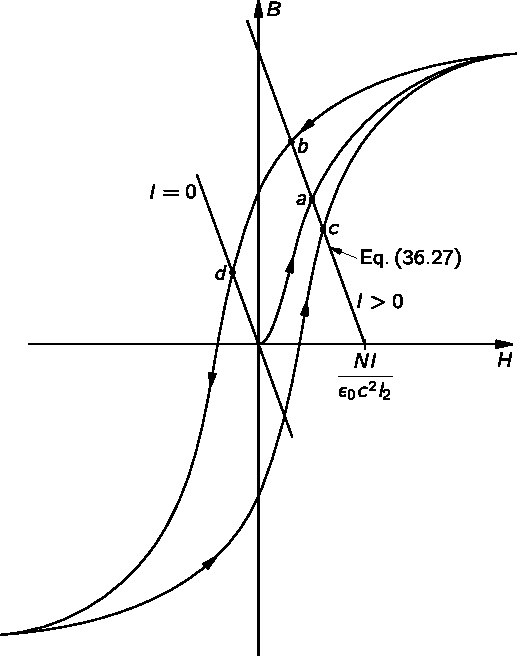
\includegraphics[width=0.7\linewidth]{fyz_fig0842.pdf}
      \caption{
               (\cite[s.~707]{Feynman02})}
      \label{fyz:fig0842}
    \end{figure}

    \begin{figure}[ht!] %\ref{fyz:fig0843}
      \centering
      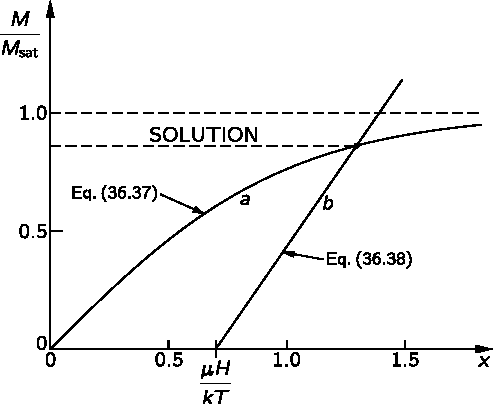
\includegraphics[width=0.7\linewidth]{fyz_fig0843.pdf}
      \caption{
               (\cite[s.~707]{Feynman02})}
      \label{fyz:fig0843}
    \end{figure}

    \begin{figure}[ht!] %\ref{fyz:fig0844}
      \centering
      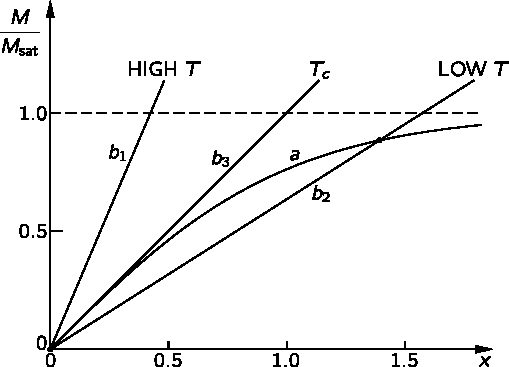
\includegraphics[width=0.7\linewidth]{fyz_fig0844.pdf}
      \caption{
               (\cite[s.~707]{Feynman02})}
      \label{fyz:fig0844}
    \end{figure}

    \begin{figure}[ht!] %\ref{fyz:fig0845}
      \centering
      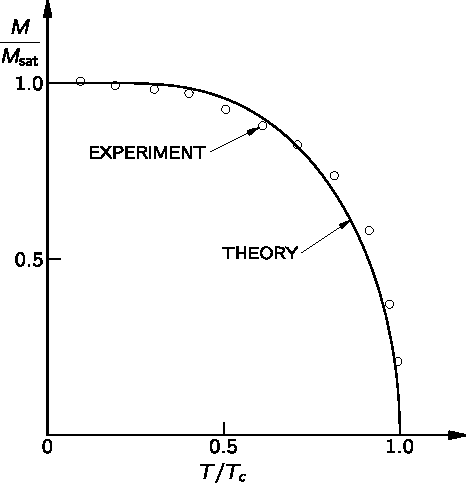
\includegraphics[width=0.7\linewidth]{fyz_fig0845.pdf}
      \caption{
               (\cite[s.~707]{Feynman02})}
      \label{fyz:fig0845}
    \end{figure}

    \todo[inline]{Kapitola fey1ch36 je zcela prázdná, pouze obrázky}  
%} %tikzset
%---------------------------------------------------------------------------------------------------